\documentclass{article}
%\usepackage[latin1]{inputenc}
\usepackage{graphicx,amssymb,amsmath,amsbsy} % extensions pour maths avancées
\usepackage{graphicx}           % extensions pour figures
\usepackage[T1]{fontenc}        % pour les charactères accentués 
\usepackage[utf8]{inputenc} 

\usepackage{stmaryrd} % Pour les crochets d'ensemble d'entier
\usepackage{float}  % Pour placer les images là ou JE veux.

\DeclareMathOperator{\tr}{tr}
\DeclareMathOperator{\argmax}{argmax}


\setlength{\parindent}{0.0in}
\setlength{\parskip}{0.3in}
\setlength{\topmargin}{-0.4in}
\setlength{\topskip}{1in}    % between header and text
\setlength{\textheight}{8in} % height of main text
\setlength{\textwidth}{4.5in}    % width of text
\setlength{\oddsidemargin}{1in} % odd page left margin
\setlength{\evensidemargin}{1in} % even page left margin
%
%% Quelques raccourcis clavier :
\def\slantfrac#1#2{\kern.1em^{#1}\kern-.3em/\kern-.1em_{#2}}
\def\b#1{\mathbf{#1}}
\def\bs#1{\boldsymbol{#1}}
\def\m#1{\mathrm{#1}}
%
\newcommand{\greeksym}[1]{{\usefont{U}{psy}{m}{n}#1}}
\newcommand{\inc}{\mbox{\small\greeksym{d}\hskip 0.05ex}}%
\pagenumbering{arabic}
\date{\today}
\title{Modèles Graphiques}
\author{Barbara Gris \& Nelle Varoquaux}
\begin{document}
\maketitle
\tableofcontents{}
\vfill \eject


\section{Apprentissage dans les modèles discrets}
Soit $z$ et $x$ deux variables aléatoires pouvant prendre
respectivement $N$ et $K$ valeurs telles que: $p(z= m) =
\pi_m$ et $p(x=k|z=m) = \theta_{m,k}$

On suppose que l'on observe $n$ valeurs $(x_i, z_i)$ iid. On note 
$N_{i, j}$ le cardinal de 
$\{k \in \llbracket 1, n \rrbracket | (x_{k}, z_k) = (j, i)\}$ et $N_i$ celui
de $\{j \in \llbracket 1, n \rrbracket | z_j = i \}$.

L'estimateur $(\pi, \theta)$ du maximum de vraisemblance est:

$(\pi, \theta) = \argmax \{ \prod_{k=1}^n p(x_k, z_k) | \sum_{i=1}^{M}\pi_{i}=1; \forall m,\sum_{k=1}^{K}\theta_{m,k}=1 \}$

$(\pi, \theta) = \argmax \{ \prod_{i=1}^M \prod_{j=1}^K \pi_i^{N_ij} \theta_{i,j}^{N_{ij}} | \sum_{i=1}^{M}\pi_{i}=1; \forall m,\sum_{k=1}^{K}\theta_{m,k}=1 \}$

$(\pi, \theta) = \argmax \{\sum_{i=1}^{M} \sum_{j=1}^K N_{i,j}(\log\pi_{i} + \log(\theta_{i,j})| \sum_{i=1}^{M}\pi_{i}=1; \forall m,\sum_{k=1}^{K}\theta_{m,k}=1 \}$

$(\pi, \theta) = \argmax \{\sum_{i=1}^{M} \sum_{j=1}^K N_{i,j}\log\pi_{i} + \sum_{i=1}^{M} \sum_{j=1}^K n_{i,j}\log(\theta_{i,j}| \sum_{i=1}^{M}\pi_{i}=1; \forall m,\sum_{k=1}^{K}\theta_{m,k}=1 \}$

$(\pi, \theta) = \argmax \{\sum_{i=1}^{M} \sum_{j=1}^K N_{i,j}\log\pi_{i} + \sum_{i=1}^{M} \sum_{j=1}^K N_{i,j}\log\theta_{i,j} | \sum_{i=1}^{M}\pi_{i}=1; \forall m,\sum_{k=1}^{K}\theta_{m,k}=1 \}$

Comme la première double somme ne dépend que de $\pi$ et la deuxième que de $\theta$, on peut calculer les valeurs pour lesquelles elles sont maximales séparément, on a donc:
$$\pi = \argmax \{\sum_{i=1}^{M} \sum_{j=1}^K N_{i,j} \log\pi_i| \sum_{i=1}^{M}\pi_{i}=1 \}$$
$$\pi=\argmax \{\sum_{i=1}^{M}  N_{i} \log\pi_i| \sum_{i=1}^{M}\pi_{i}=1 \}$$
et
$$\theta = (\theta_1, ... \theta_M)$$

avec $\theta_i = \argmax \{ \sum_{j=1}^K N_{i,j}\log\theta_{i,j}|\forall m,\sum_{k=1}^{K}\theta_{m,k}=1 \}$



\subsection{Calcul du maximum de vraisemblance de $\pi$}
On utilise la méthode du lagrangien.\\

On note donc $\mathcal{L}(\pi, \lambda) = \sum_{i=1}^{M} (N_{i} \log \pi_{i}) + \lambda((\sum_{i=1}^{M}\pi_{i})-1)$\\

 $\mathcal{L}(\pi, \lambda)=\sum_{i=1}^{M} (N_{i} \log\pi_{i}+\lambda\pi_{i}+\frac{\lambda}{M})$.\\
 Comme le i-ème terme de la somme ne dépend que de $\pi_{i}$, pour maximiser
 $\mathcal{L}(\pi, \lambda)$ par rapport à $\pi_i$ il suffit de maximiser chaque i-ème terme de la somme par rapport à $\pi_i$. \\
Or $\frac{\partial}{\partial \pi_i}( N_{i} \log\pi_{i}+\lambda\pi_{i}+\frac{\lambda}{M}) = \frac{N_{i}}{\pi_i} + \lambda$ donc cette dérivée est nulle $ssi$ $\pi_i=-\frac{N_i}{\lambda}$, négative pour $\pi_i>-\frac{N_i}{\lambda}$ et positive sinon. 

Ainsi $\frac{\partial (N_{i}
\log\pi_{i}+\lambda\pi_{i}+\frac{\lambda}{M})}{\partial \pi_i}$ est maximal en $\pi_i=-\frac{N_i}{\lambda}$. Donc à $\lambda$ fixé, $\mathcal{L}(\pi, \lambda)$ est maximal pour $\hat{\pi}(\lambda)=(-\frac{N_1}{\lambda}, ..., -\frac{N_M}{\lambda})$.

De plus comme $\min\{\mathcal{L}(\hat{\pi}(\lambda),
\lambda)|\lambda\in\Re\} = \max \{\sum_{i=1}^{M} \sum_{j=1}^K N_{i,j} \log\pi_i| \sum_{i=1}^{M}\pi_{i}=1 \}$ et que ce minimum est atteint pour $\lambda $ tel que $\sum_{i=1}^{M}\hat{\pi}(\lambda)_i=1$, il est atteint pour $\lambda = -n$ et donc finalement l'estimateur du maximum de vraisemblance de $\pi$ est $$\hat{\pi}=(\frac{N_1}{n}, ..., \frac{N_M}{n}).$$


\subsection{Maximum de Vraisemblance de $\theta$}
De même que précédemment on peut calculer les valeurs de $\theta_{i}=(\theta_{i,1}, ..., \theta_{i,K})$ pour lesquelles $\sum_{j=1}^K N_{i,j}\log\theta_{i,j}$ est maximale avec $\forall m,\sum_{k=1}^{K}\theta_{m,k}=1$ séparément.
Un calcul analogue à celui de la partie précédente montre alors que $\hat{\theta}_{i}=(\frac{N_{i,1}}{n}, ..., \frac{N_{i,K}}{n})$

\section{Classification linéaire}
\subsection{1.Modèle génératif (LDA)}

On suppose que l'on observe $N$ valeurs $(x_i, y_i)$ iid. Calculons le maximum de vraisemblance de $\theta=(\pi, \Sigma, \mu_0, \mu_1)$.

La log-vraisemblance est par définition:

$l(\theta) = \log(\prod_{n=1}^N p (y_n | \pi)  p(x_{ n}|y_n, \theta))$

$l(\theta) = \sum_{n=1}^N \log p(y_n |\pi) + \sum_{n=1}^{N} \log p(x_{ n}|y_n,  \Sigma, \mu_0, \mu_1)$

On peut donc maximiser le premier terme indépendamment du deuxième terme.

La valeur de $\pi$ pour laquelle le premier terme est maximal a déjà été calculé dans l'exercice 1 : l'estimateur du maximum de vraisemblance de $\pi$ est $$\hat{\pi} = \frac{\sum_{n=1}^{N} y_{n}}{N}.$$

Le deuxième terme s'écrit:

$l(\theta) = \sum_{n=1}^{N} \log(\frac{1}{2\pi|\Sigma|^{1/2}} (\exp(-\frac{1}{2}(x_{n}-\mu_{1})^{T}\Sigma^{-1}(x_{n}-\mu_{1})))^{y_{n}}(\exp(-\frac{1}{2}(x_{n}-\mu_{0})^{T}\Sigma^{-1}(x_{n}-\mu_{0})))^{1-y_{n}}$ \\
$l(\theta) = \sum_{n=1}^{N} (\log(\frac{1}{2\pi|\Sigma|^{1/2}})-\frac{y_{n}}{2}(x_{n}-\mu_{1})^{T}\Sigma^{-1}(x_{n}-\mu_{1})-\frac{1-y_{n}}{2}(x_{n}-\mu_{0})^{T}\Sigma^{-1}(x_{n}-\mu_{0}))$.

\subsubsection{Estimation de $\mu_1$ et $\mu_0$}
$l( \Sigma, \mu_0, \mu_1) $ ne dépend de $ \mu_1$ que par $l_{1}=\sum_{n=1}^{N}-\frac{y_{n}}{2}(x_{n}-\mu_{1})^{T}\Sigma^{-1}(x_{n}-\mu_{1})$ donc la valeur de $ \mu_1$ pour laquelle cette quantité est maximale est également celle qui maximise $l( \Sigma, \mu_0, \mu_1) $ (par rapport à $\mu_1$).\\
Or $\nabla_{\mu_{1}}l_{1}=2\sum_{n=1}^{N}y_{n}(x_{n}+\mu_{1})^{T}\Sigma^{-1}$ donc ce gradient s'annule pour $\mu_{1}=\frac{\sum{n=1}^{N}y_{n}x_{n}}{\sum_{n=1}^{N}y_{n}}$.\\
Ainsi l'estimateur du maximum de vraisemblance de $\mu_{1}$ est $$\hat{\mu}_{1}=\frac{\sum_{n=1}^{N}y_{n}x_{n}}{\sum_{n=1}^{N}y_{n}}$$
et de même $$\hat{\mu}_{0}=\frac{\sum_{n=1}^{N}(1-y_{n})x_{n}}{\sum_{n=1}^{N}1-y_{n}}.$$

\subsubsection{Estimation de $\Sigma$}
Il faut maximiser $l( \Sigma, \hat{\mu_0}, \hat{\mu_1})$ par rapport à
$\Sigma$. On pose $\Gamma=\Sigma^{-1}$ et on maximise $l( \Gamma, \hat{\mu_0}, \hat{\mu_1}) $ par rapport à $\Gamma$.\\
Le gradient de $l$ en $\Gamma$ est $$\nabla_{\Gamma}l=\frac{1}{2} \sum_{n=1}^{N}(\Gamma^{-1}-y_{n}(x_{n}-\hat{\mu_{1}})(x_{n}-\hat{\mu_{1}})^{T}-(1-y_{n})(x_{n}-\hat{\mu_{0}})(x_{n}-\hat{\mu_{0}})^{T})$$
donc ce gradient s'annule pour $$\Gamma^{-1} = \frac{\sum_{n=1}^{N} ( y_{n}(x_{n}-\hat{\mu_{1}})(x_{n}-\hat{\mu_{1}})^{T}+(1-y_{n})(x_{n}-\hat{\mu_{0}})(x_{n}-\hat{\mu_{0}})^{T})}{N}.$$
Ainsi l'estimateur du maximum de vraisemblance de $\Sigma$ est $$\hat{\Sigma} = \frac{\sum_{n=1}^{N} ( y_{n}(x_{n}-\hat{\mu_{1}})(x_{n}-\hat{\mu_{1}})^{T}+(1-y_{n})(x_{n}-\hat{\mu_{0}})(x_{n}-\hat{\mu_{0}})^{T})}{N}.$$

\subsection{Comparaison des trois modèles}


\begin{tabular}{| c | l | l | l |}
          & LDA & Régression Logistique & Régression Linéaire \\
A         & 0.216667 & \textbf{0.16}    & \textbf{0.16}      \\
B         & 0.126667 & 0.1     & \textbf{0.08333}   \\
C         & 0.155    & \textbf{0.12}    & 0.16       \\
\end{tabular}

\begin{figure}[h]
\caption{Training data A}
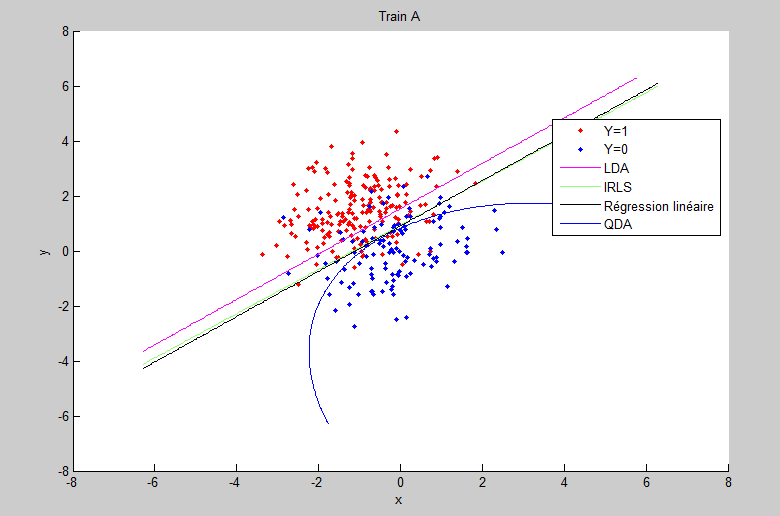
\includegraphics[width=300px]{TrainA.png}
\end{figure}

\paragraph{Jeu de données A}

Le barycentre des données est équidistant des nuages de points $Y = 0$ et $Y =
1$, ce qui explique la bonne performance de la régression linéaire. En effet,
plus un point est éloigné du barycentre, plus il a de poids. Ici, les points
de classe $Y = 0$ ont donc à peu près le même poids que ceux de classe $Y =
0$. Bien que les deux ensembles de points ne soient pas très bien séparés, la
régression linéaire maximise facilement la bonne classification des données de
tests.

Entre LDA et IRLS, la pente des droites est très proche, mais la constante
varie. IRLS est une méthode d'approximation itérative, qui suit le même
principe que LMS (least mean square), qui converge très bien pour la
régression linéaire. Comme cette dernière est très efficace ici, il n'est donc
pas surprenant qu'IRLS marche si bien sur ces données.

On peut supposer que si il y a un biais dans les données, il sera plus
facilement corrigé par un algorithme itératif (IRLS) que par un calcul direct
(LDA). Cela peut expliquer le plus faible taux d'erreur pour IRLS que pour
LDA.

\begin{figure}[H]
\caption{Test data A}
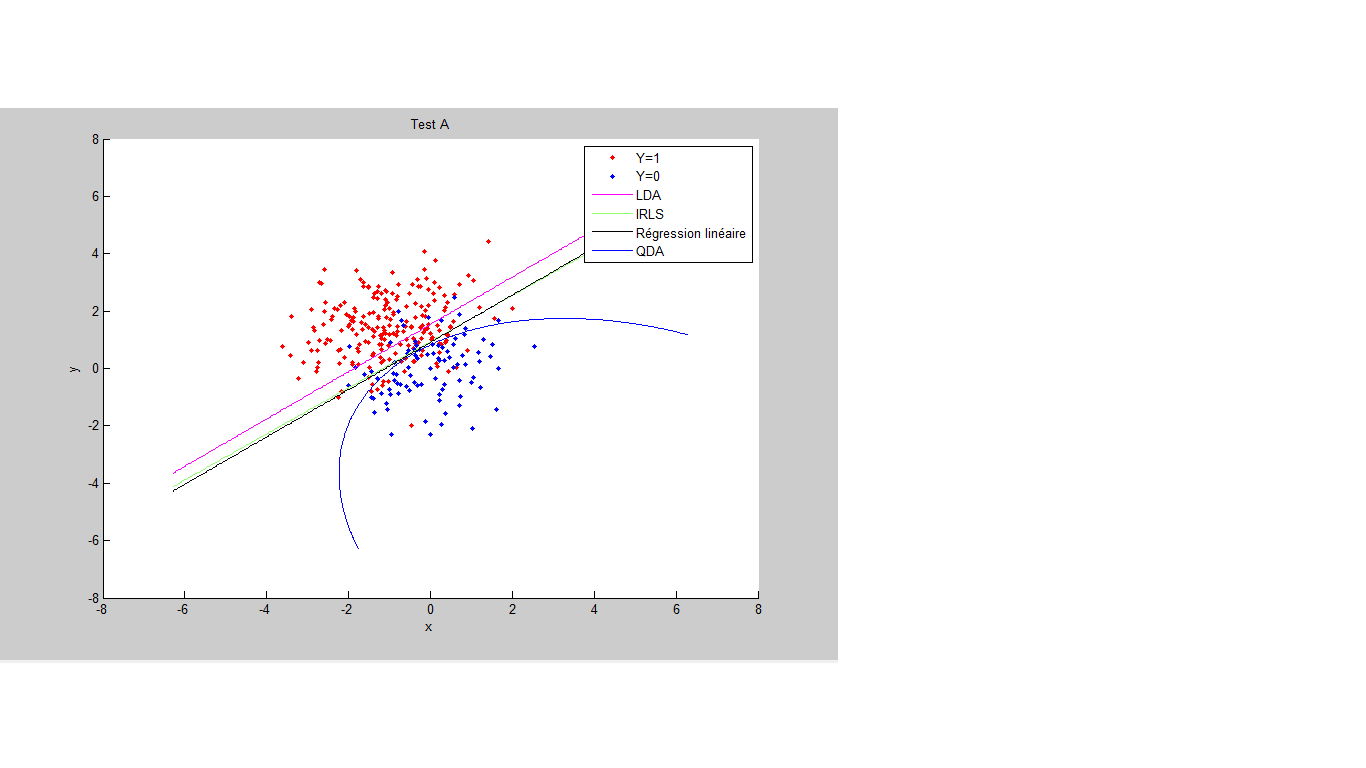
\includegraphics[width=300px]{TestA.png}
\end{figure}

\begin{figure}[h]
\caption{Training data B}
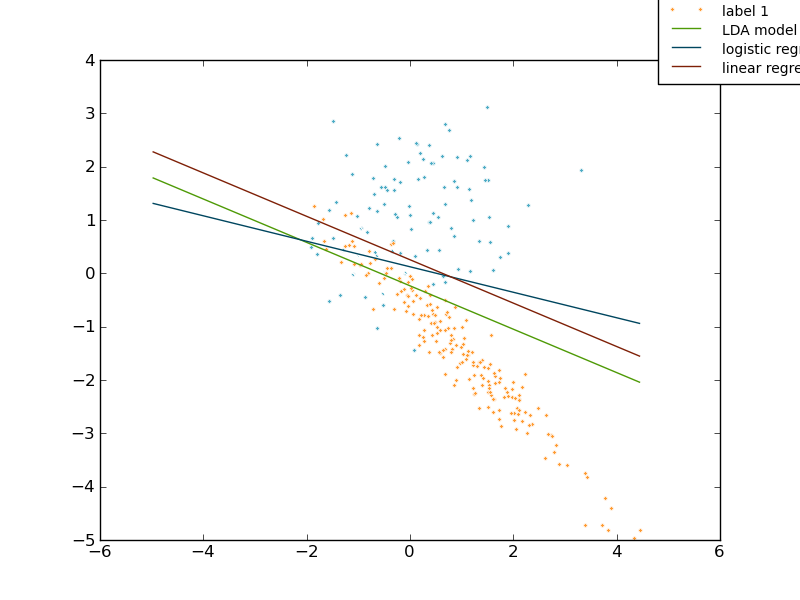
\includegraphics[width=300px]{classificationB1.png}
\end{figure}

\paragraph{Jeu de tests B}

La régression linéaire fonctionne très bien sur ce jeu de données, car les
points tels que $Y = 1$ sont visuellement proches d'une droite, qui est elle
même orthogonal à la moyenne des vecteurs pour $Y = 0$. Ainsi il semble
réaliste de trouver un vecteur $\theta$ tel que pour le point X tel que $Y = 1$,
$\theta X = 1$, et dans l'autre cas $\theta X = 0$

On remarque que les deux autres méthodes sont aussi relativement bonnes. Ce
n'est pas surprenant, les données étant visuellement séparées.

\begin{figure}[H]
\caption{Test data B}
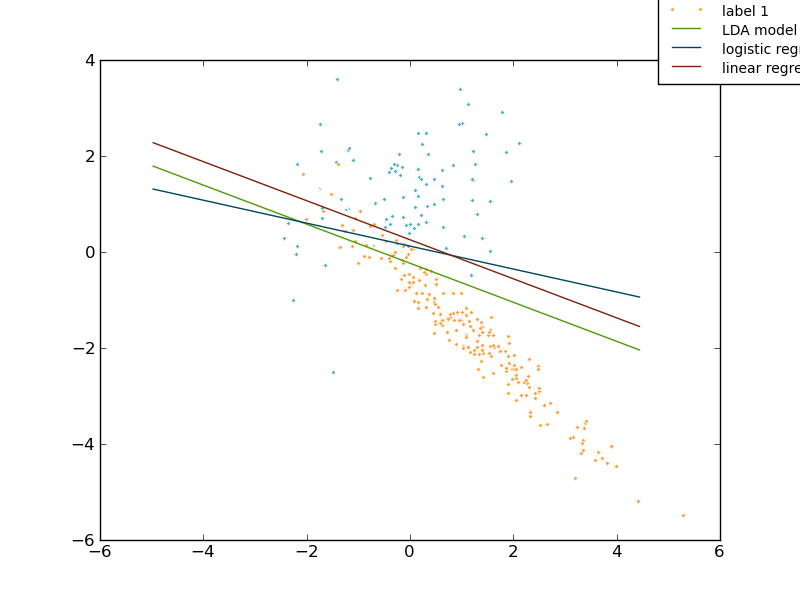
\includegraphics[width=300px]{classificationB1_test.png}
\end{figure}


\begin{figure}[H]
\caption{Test data B}
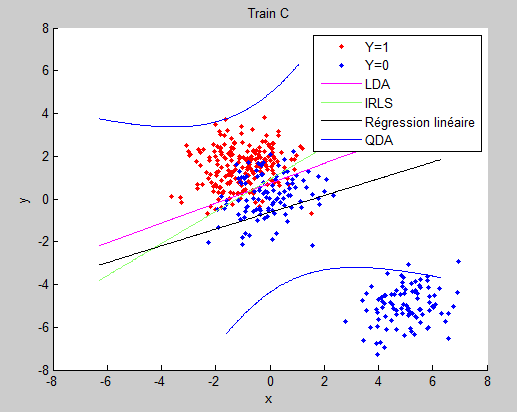
\includegraphics[width=300px]{TrainC.png}
\end{figure}

\paragraph{Jeu de tests C}

Les points sont visuellement proche d'une même droite. Si un vecteur $\theta$
est tel que $\theta X = 1$ pour $Y = 1$, alors pour une grande partie des
points tels que $Y = 0$, on aura aussi $\theta X = 1$. Pour la régression
linéaire, la distance au barycentre des points joue énormement (mauvais
traitement des données bimodales). Même les points exceptionnellement éloignés
du barycentre ont une importance sur le calcul de theta, alors qu'ils
représentent plus du bruit. La régression linéaire est très peu robuste.

De même que pour le jeu de données B, IRLS et LDA donnent des résultats tout à
fait satisfaisants.

\begin{figure}[H]
\caption{Test data B}
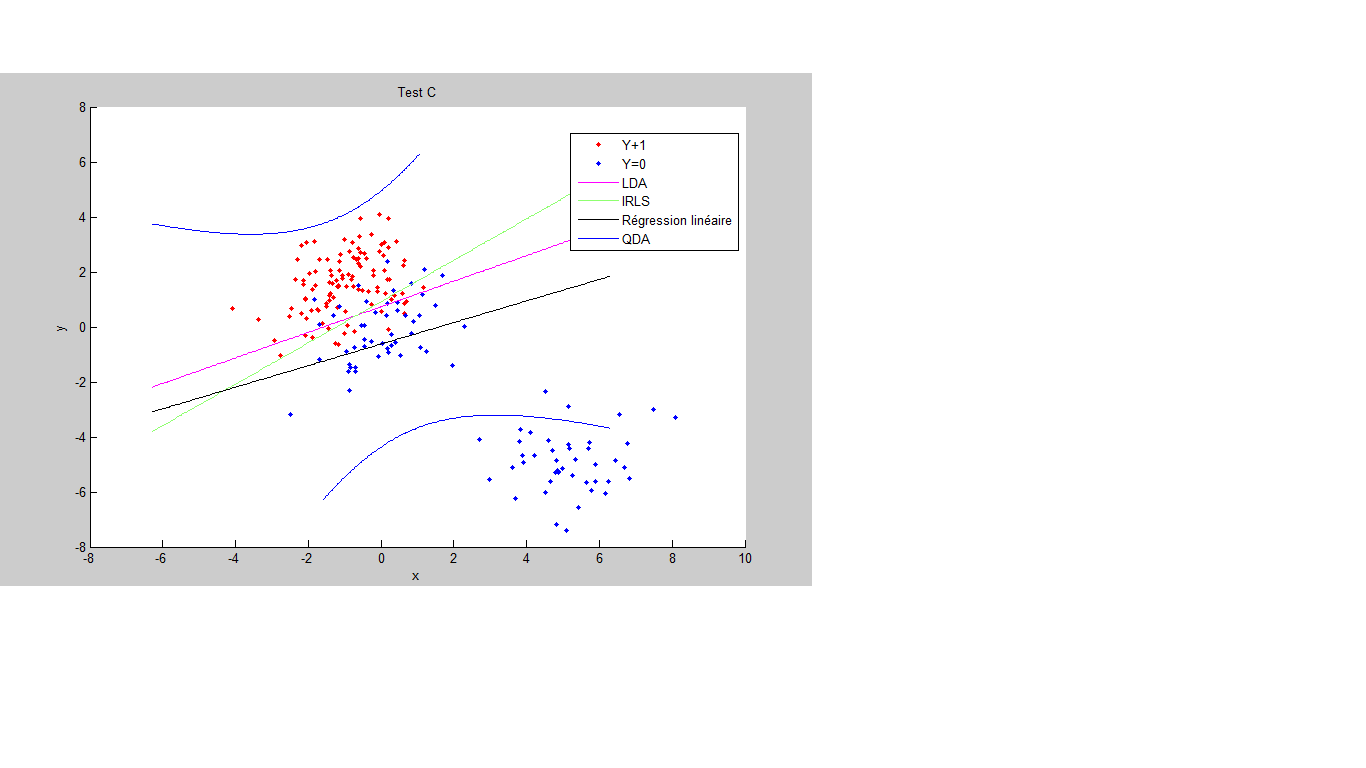
\includegraphics[width=300px]{TestC.png}
\end{figure}


\subsection{5.Modèle génératif (QDA)}
\subsubsection{Maximum de vraisemblance }
On suppose que l'on observe $N$ valeurs $(x_i, y_i)$ iid. Calculons le maximum de vraisemblance de $\theta=(\pi, \Sigma_{0}, \Sigma_{1}, \mu_0, \mu_1)$.

La log-vraisemblance est par définition:

$l(\theta) = \log(\prod_{n=1}^N p (y_n | \pi)  p(x_{ n}|y_n, \theta))$

$l(\theta) = \sum_{n=1}^N \log(p(y_n |\pi)) + \sum_{n=1}^{N} \log(p(x_{ n}|y_n,  \Sigma_{0}, \Sigma_{1}, \mu_0, \mu_1))$

On peut donc maximiser le premier terme indépendamment du deuxième terme.

D'après l'exercice 1, l'estimateur du maximum de vraisemblance de $\pi$ est $$\hat{\pi} = \frac{\sum_{n=1}^{N} y_{n}}{N}.$$

Le deuxième terme s'écrit:

$l(\Sigma_{0}, \Sigma_{1}, \mu_0, \mu_1) = \sum_{n=1}^{N} \log(\frac{1}{2\pi}\frac{1}{|\Sigma_{1}|^{\frac{y_{n}}{2}}}\frac{1}{|\Sigma_{0}|^{\frac{1-y_{n}}{2}}} (\exp(-\frac{1}{2}(x_{n}-\mu_{1})^{T}\Sigma_{1}^{-1}(x_{n}-\mu_{1})))^{y_{n}}(\exp(-\frac{1}{2}(x_{n}-\mu_{0})^{T}\Sigma_{0}^{-1}(x_{n}-\mu_{0})))^{1-y_{n}}$ \\ \\
$l(\Sigma_{0}, \Sigma_{1}, \mu_0, \mu_1) = \sum_{n=1}^{N} (\log(\frac{1}{2\pi})-\frac{y_{n}}{2}\log(|\Sigma_{1}|)-\frac{1-y_{n}}{2}\log(|\Sigma_{0}|)-\frac{y_{n}}{2}(x_{n}-\mu_{1})^{T}\Sigma_{1}^{-1}(x_{n}-\mu_{1})-\frac{1-y_{n}}{2}(x_{n}-\mu_{0})^{T}\Sigma-{0}^{-1}(x_{n}-\mu_{0}))$.\\
Les estimateurs de $\mu_0$ et $\mu_1$ se calculent de la même manière qu'à la question 1.\\\\
$l(\Sigma_{0}, \Sigma_{1}, \mu_0, \mu_1)$ ne dépend de $\Sigma_{1}$ que par $l_{2}=\sum_{n=1}^{N}(-\frac{y_{n}}{2}\log(|\Sigma_{1}|))-\frac{y_{n}}{2}(x_{n}- \hat {\mu}_{1})^{T}\Sigma_{1}^{-1}(x_{n}-\hat {\mu}_{1})$. \\
On pose $\Gamma_{1} = \Sigma_1$ et on maximise $l_{2}$ en fonction de $\Gamma_{1}$. \\
$\nabla_{\Gamma_{1}}l_{2}= \frac{1}{2}(\sum_{n=1}^{N}y_{n})\Gamma^{-1}-\frac{1}{2}\sum_{n=1}^{N}(y_{n}(x_{n}-\mu_{1})(x_{n}-\mu_{1})^{T})$\\
donc ce gradient s'annule pour $\Gamma^{-1}=\frac{\sum_{n=1}^{N}(y_{n}(x_{n}-\mu_{1})(x_{n}-\mu_{1})^{T})}{\sum_{n=1}^{N}y_{n}}$.\\
Ainsi l'estimateur du maximum de vraisemblance de $\Sigma_{1}$ est 
$$\hat{\Sigma}_{1} = \frac{\sum_{n=1}^{N}(y_{n}(x_{n}-\mu_{1})(x_{n}-\mu_{1})^{T})}{\sum_{n=1}^{N}y_{n}}.$$
De même, on montre que $$\hat{\Sigma}_{0} = \frac{\sum_{n=1}^{N}((1-y_{n})(x_{n}-\mu_{0})(x_{n}-\mu_{0})^{T})}{\sum_{n=1}^{N}1-y_{n}}.$$

\subsubsection{Conique d'équation $p(y=1|x)=0.5$}
D'après la formule de Bayes:\\
$p(y=1|x)=\frac{p(x|y=1)p(y=1)}{p(x)}$\\\\
$p(y=1|x)=\frac{\frac{\pi}{|\Sigma_{1}|}\exp(-\frac{1}{2}(x-\mu_{1})^{T}\Sigma_{1}^{-1}(x-\mu_{1}))}{\frac{\pi}{|\Sigma_{1}|}\exp(-\frac{1}{2}(x-\mu_{1})^{T}\Sigma_{1}^{-1}(x-\mu_{1})) + \frac{\pi}{|\Sigma_{0}|}\exp(-\frac{1}{2}(x-\mu_{0})^{T}\Sigma_{0}^{-1}(x-\mu_{0}))}$\\\\
$p(y=1|x)=\frac{1}{1+\exp(\log(\frac{1-\pi}{\pi})+\frac{1}{2}((x-\mu_{1})^{T}\Sigma_{1}^{-1}(x-\mu_{1}) - (x-\mu_{0})^{T}\Sigma_{0}^{-1}(x-\mu_{0})}$\\\\
Ainsi $p(y=1|x)=0.5$ $ssi$ $\log(\frac{1-\pi}{\pi})+\frac{1}{2}((x-\mu_{1})^{T}\Sigma_{1}^{-1}(x-\mu_{1}) - (x-\mu_{0})^{T}\Sigma_{0}^{-1}(x-\mu_{0}) = 0$ ce qui définit bien une conique.


\end{document}
